% Options for packages loaded elsewhere
\PassOptionsToPackage{unicode}{hyperref}
\PassOptionsToPackage{hyphens}{url}
%
\documentclass[
]{article}
\usepackage{lmodern}
\usepackage{amssymb,amsmath}
\usepackage{ifxetex,ifluatex}
\ifnum 0\ifxetex 1\fi\ifluatex 1\fi=0 % if pdftex
  \usepackage[T1]{fontenc}
  \usepackage[utf8]{inputenc}
  \usepackage{textcomp} % provide euro and other symbols
\else % if luatex or xetex
  \usepackage{unicode-math}
  \defaultfontfeatures{Scale=MatchLowercase}
  \defaultfontfeatures[\rmfamily]{Ligatures=TeX,Scale=1}
\fi
% Use upquote if available, for straight quotes in verbatim environments
\IfFileExists{upquote.sty}{\usepackage{upquote}}{}
\IfFileExists{microtype.sty}{% use microtype if available
  \usepackage[]{microtype}
  \UseMicrotypeSet[protrusion]{basicmath} % disable protrusion for tt fonts
}{}
\makeatletter
\@ifundefined{KOMAClassName}{% if non-KOMA class
  \IfFileExists{parskip.sty}{%
    \usepackage{parskip}
  }{% else
    \setlength{\parindent}{0pt}
    \setlength{\parskip}{6pt plus 2pt minus 1pt}}
}{% if KOMA class
  \KOMAoptions{parskip=half}}
\makeatother
\usepackage{xcolor}
\IfFileExists{xurl.sty}{\usepackage{xurl}}{} % add URL line breaks if available
\IfFileExists{bookmark.sty}{\usepackage{bookmark}}{\usepackage{hyperref}}
\hypersetup{
  hidelinks,
  pdfcreator={LaTeX via pandoc}}
\urlstyle{same} % disable monospaced font for URLs
\usepackage{color}
\usepackage{fancyvrb}
\newcommand{\VerbBar}{|}
\newcommand{\VERB}{\Verb[commandchars=\\\{\}]}
\DefineVerbatimEnvironment{Highlighting}{Verbatim}{commandchars=\\\{\}}
% Add ',fontsize=\small' for more characters per line
\newenvironment{Shaded}{}{}
\newcommand{\AlertTok}[1]{\textcolor[rgb]{1.00,0.00,0.00}{\textbf{#1}}}
\newcommand{\AnnotationTok}[1]{\textcolor[rgb]{0.38,0.63,0.69}{\textbf{\textit{#1}}}}
\newcommand{\AttributeTok}[1]{\textcolor[rgb]{0.49,0.56,0.16}{#1}}
\newcommand{\BaseNTok}[1]{\textcolor[rgb]{0.25,0.63,0.44}{#1}}
\newcommand{\BuiltInTok}[1]{#1}
\newcommand{\CharTok}[1]{\textcolor[rgb]{0.25,0.44,0.63}{#1}}
\newcommand{\CommentTok}[1]{\textcolor[rgb]{0.38,0.63,0.69}{\textit{#1}}}
\newcommand{\CommentVarTok}[1]{\textcolor[rgb]{0.38,0.63,0.69}{\textbf{\textit{#1}}}}
\newcommand{\ConstantTok}[1]{\textcolor[rgb]{0.53,0.00,0.00}{#1}}
\newcommand{\ControlFlowTok}[1]{\textcolor[rgb]{0.00,0.44,0.13}{\textbf{#1}}}
\newcommand{\DataTypeTok}[1]{\textcolor[rgb]{0.56,0.13,0.00}{#1}}
\newcommand{\DecValTok}[1]{\textcolor[rgb]{0.25,0.63,0.44}{#1}}
\newcommand{\DocumentationTok}[1]{\textcolor[rgb]{0.73,0.13,0.13}{\textit{#1}}}
\newcommand{\ErrorTok}[1]{\textcolor[rgb]{1.00,0.00,0.00}{\textbf{#1}}}
\newcommand{\ExtensionTok}[1]{#1}
\newcommand{\FloatTok}[1]{\textcolor[rgb]{0.25,0.63,0.44}{#1}}
\newcommand{\FunctionTok}[1]{\textcolor[rgb]{0.02,0.16,0.49}{#1}}
\newcommand{\ImportTok}[1]{#1}
\newcommand{\InformationTok}[1]{\textcolor[rgb]{0.38,0.63,0.69}{\textbf{\textit{#1}}}}
\newcommand{\KeywordTok}[1]{\textcolor[rgb]{0.00,0.44,0.13}{\textbf{#1}}}
\newcommand{\NormalTok}[1]{#1}
\newcommand{\OperatorTok}[1]{\textcolor[rgb]{0.40,0.40,0.40}{#1}}
\newcommand{\OtherTok}[1]{\textcolor[rgb]{0.00,0.44,0.13}{#1}}
\newcommand{\PreprocessorTok}[1]{\textcolor[rgb]{0.74,0.48,0.00}{#1}}
\newcommand{\RegionMarkerTok}[1]{#1}
\newcommand{\SpecialCharTok}[1]{\textcolor[rgb]{0.25,0.44,0.63}{#1}}
\newcommand{\SpecialStringTok}[1]{\textcolor[rgb]{0.73,0.40,0.53}{#1}}
\newcommand{\StringTok}[1]{\textcolor[rgb]{0.25,0.44,0.63}{#1}}
\newcommand{\VariableTok}[1]{\textcolor[rgb]{0.10,0.09,0.49}{#1}}
\newcommand{\VerbatimStringTok}[1]{\textcolor[rgb]{0.25,0.44,0.63}{#1}}
\newcommand{\WarningTok}[1]{\textcolor[rgb]{0.38,0.63,0.69}{\textbf{\textit{#1}}}}
\usepackage{graphicx,grffile}
\makeatletter
\def\maxwidth{\ifdim\Gin@nat@width>\linewidth\linewidth\else\Gin@nat@width\fi}
\def\maxheight{\ifdim\Gin@nat@height>\textheight\textheight\else\Gin@nat@height\fi}
\makeatother
% Scale images if necessary, so that they will not overflow the page
% margins by default, and it is still possible to overwrite the defaults
% using explicit options in \includegraphics[width, height, ...]{}
\setkeys{Gin}{width=\maxwidth,height=\maxheight,keepaspectratio}
% Set default figure placement to htbp
\makeatletter
\def\fps@figure{htbp}
\makeatother
\setlength{\emergencystretch}{3em} % prevent overfull lines
\providecommand{\tightlist}{%
  \setlength{\itemsep}{0pt}\setlength{\parskip}{0pt}}
\setcounter{secnumdepth}{-\maxdimen} % remove section numbering

\date{}

\begin{document}

\hypertarget{header-n0}{%
\section{Dec 5 Thu}\label{header-n0}}

\hypertarget{header-n2}{%
\subsection{SE-344::CG}\label{header-n2}}

\hypertarget{header-n3}{%
\subsubsection{NURBS}\label{header-n3}}

NURBS 看起来很眼熟\ldots3ds max 里似乎有叫这个名字的功能。

翻译成人话就是非均匀有理 B 样条曲线。换句话说,他也是上面我们提到的 B
样条曲线的一种。

\hypertarget{header-n6}{%
\paragraph{特征}\label{header-n6}}

\begin{itemize}
\item
  非均匀
\item
  有理
\end{itemize}

所谓非均匀的意思就是,每个节点分量在参数轴上的分布非均匀。

也就是说,每个控制顶点不再平等了,他们可能会拥有不同的权重,对整体曲线的影响力也就不同。

\begin{figure}
\centering

\includegraphics{/Users/yue/Documents/GitHub/2019-2020-autumn-semester/SE-344/submissions/ass4-ng-x/notes/12-05.assets/image-20191229160650098.png}
\caption{}
\end{figure}

在函数中的表示,就是增加了一个权重分量 \texttt{W}。

\hypertarget{header-n16}{%
\paragraph{优点}\label{header-n16}}

\begin{itemize}
\item
  投影变换/仿射变换下都保持不变
\item
  相比均匀的 B 样条曲线更灵活
\item
  ISO 认证,唯一表示法
\item
  高度直觀性和可預測性
\end{itemize}

\begin{quote}
控制点看起来要么跟最终的结果直接相连,要么表现起来跟结果用一根「橡皮筋」相连。
\end{quote}

\hypertarget{header-n28}{%
\paragraph{缺点}\label{header-n28}}

\begin{itemize}
\item
  运算耗时长
\item
  权重决定不好选,选错了问题大
\item
  点的映射算法在 NURBS 下不稳定(???)
\end{itemize}

\begin{quote}
?为什么不稳定?

正向运算肯定是稳定的,也就是说通过各个参数值求出实际点位置肯定稳。

而反向运算跟均匀的 B 样条有什么区别呢?

非均匀。就是因为非均匀,计算上耗时肯定没那么方便了。

况且,鉴于权值分布不均匀,必然存在一些控制柄的权值低于平均,在反求他们的参数的时候,较小的误差就可能带来较大的不同。这种误差可能来自采样精度、浮点数运算精度等等。

无法逆运算是个比较致命的问题。
\end{quote}

\hypertarget{header-n43}{%
\subsubsection{Draw Bezier}\label{header-n43}}

道理我都懂了,但是 OpenGL 怎么画曲线?

\hypertarget{header-n45}{%
\paragraph{首先}\label{header-n45}}

打开一些神秘宏定义的开关(这种开关在 OpenGL 里可太多了)

\begin{Shaded}
\begin{Highlighting}[]
\NormalTok{glEnable(GL_MAP1_VERTEXT_3);}
\NormalTok{glEnable(GL_MAP1_TEXTURE_COORD_3);}
\end{Highlighting}
\end{Shaded}

\hypertarget{header-n48}{%
\paragraph{然后}\label{header-n48}}

调用 \texttt{glEvalCoord1f}
函数来确认在不同的参数取值下,对应到结果曲线的坐标。

\hypertarget{header-n50}{%
\paragraph{最后}\label{header-n50}}

用 \texttt{glBegin(GL\_LINE\_STRIP)} 开始把这些点连成折线。

虽然本质上是折线\ldots\ldots 但是呢,函数帮我们算好了非常贴近 Bezier
曲线的点序列,把他们画出来看起来就是那么回事了。

\hypertarget{header-n53}{%
\paragraph{Draw NURBS}\label{header-n53}}

看起来 Bezier 曲线满含酸的\ldots 连独立的 API
都没有,对应的工具函数只是做数学计算。最后还要我们自己画折线(伪·曲线)。

NURBS 就不一样了:居然还有自己的类。

\begin{Shaded}
\begin{Highlighting}[]
\NormalTok{nobj= gluNewNurbsRenderer() ;}
\NormalTok{gluNurbsCallback (nobj, GLU_ERROR, ErrorCallback);}
\NormalTok{gluNurbsProperty(nobj,GLU_U_STEP,}\FloatTok{15.0}\NormalTok{ );}
\NormalTok{gluNurbsProperty(nobj,GLU_V_STEP,}\FloatTok{15.0}\NormalTok{ );}
\NormalTok{gluBeginCurve(nobj) ;}
\NormalTok{		gluNurbsCurve (nobj,…,GL_MAP1_TEXTURES_COORD_2); }
\NormalTok{		gluNurbsCurve (nobj,…,GL_MAP1_NORMAL);}
\NormalTok{		gluNurbsCurve (nobj,…,GL_VERTEX_4);}
\NormalTok{gluEndCurve (nobj);}
\end{Highlighting}
\end{Shaded}

\texttt{gluNurbsRenderer} 类型的实例创建之後,就可以通过
\texttt{gluNurbsCurve} 来声明曲线的一些信息了。

\begin{Shaded}
\begin{Highlighting}[]
\DataTypeTok{void}\NormalTok{ gluNurbsCurve (GLUnurbs *nurb,}
\NormalTok{                    GLint knotCount, }
\NormalTok{                    GLfloat *knot, }
\NormalTok{                    GLint stride, }
\NormalTok{                    GLfloat *control, }
\NormalTok{                    GLint order, }
\NormalTok{                    GLenum type)}
\end{Highlighting}
\end{Shaded}

其中,nurb 是 NURBS 对象指针; knotCount 指定 knots 中节点的数目; knots
指定一个 knotCount 的非减节点值的数组; stride
指定连续的曲线控制点之间的偏移量; control 是控制顶点数组的指针; order
是 NURBS 曲线的阶数; type 指定 NURBS 对象的类型。

\begin{quote}
这里没啥好说的\ldots 总归直接画就完了。

要讨论 API 设计的话,那 CG
里每一个都是一塌糊涂。这个复杂度没办法设计得干净。
\end{quote}

\hypertarget{header-n63}{%
\subsubsection{Line to Curve}\label{header-n63}}

从曲线到曲面:重大突破!

\hypertarget{header-n65}{%
\paragraph{参数曲面}\label{header-n65}}

参数曲面定义跟参数曲线相当类似:

参数曲线是一个参数 \(t\) 决定出一组 \((x, y)\);

而参数曲面则是两个参数 \((u, v)\) 决定出一组 \((x, y, z)\)。

反正结果就是取遍了所有的 \(t\),返回值组合在一起就能得到一根线;

取遍了所有的 \(u\) 跟 \(v\) 的组合,返回值组合在一起就拼成了一个曲面。

\hypertarget{header-n71}{%
\paragraph{连续性}\label{header-n71}}

跟参数曲线一样,参数曲面也具有 C 和 G 的连续判别法。

规则也是蛮神似的:

\begin{itemize}
\item
  假如两个曲面有公共连接线,那么他们至少 C\textsuperscript{0}
  连续,也至少 G\textsuperscript{0} 连续。
\item
  假如要求 C\textsuperscript{i}
  连续,那么要求存在一条公共连接线,在这条连接线上每一处都具有 \(i\)
  阶的连续偏导。
\item
  假如要求 G\textsuperscript{1}
  连续,那么要求存在一条公共连接线,在这条连接线上每一处都存在公共切平面。
\end{itemize}

\begin{quote}
存在公共切平面 = 存在公共的曲面法线,一码事。
\end{quote}

\begin{itemize}
\item
  那么更高级的 G 连续呢?不太好理解。
\end{itemize}

看一篇 2010 年的老文:

\begin{quote}
G0两个对象相连或两个对象的位置是连续的。G0连续(也称为点连续)在每个表面上产生一次反射,这种连续仅仅保证曲面间没有缝隙而是完全接触。
G1两个对象光顺连续,一阶微分连续,或者是相切连续的。G1连续(也称为切线连续)将产生一次完整的表面反射,反射线连续但是扭曲状,这种连续仅是方向的连续而没有半径连续。我们通常的倒圆角就是这种情况。
G2两个对象光顺连续,二阶微分连续,或者两个对象的曲率是连续的。G2连续(也称为曲率连续)将产生横过所以边界的完整的和光滑的反射纹。曲率连续意味着在任何曲面上的任一``点''中沿着边界有相同的曲率半径。外观质量要求高的产品需要曲率做到G2连续,其实曲面做到这一点难度是很大发。在我们一般的产品设计中G1连续就能满足大部分产品开发需要。
G3两的对象光顺连续,三阶微分连续等。
Gn的连续性是独立于表示(参数化)的。
\end{quote}

用简单的话说,就是 G0 - 接触,G1 - 共切线,G2 - 共曲率。

本质一点看,就是 0 阶微分,1 阶、2 阶的问题了。

\hypertarget{header-n91}{%
\paragraph{Example}\label{header-n91}}

\hypertarget{header-n92}{%
\subparagraph{平面}\label{header-n92}}

\begin{figure}
\centering
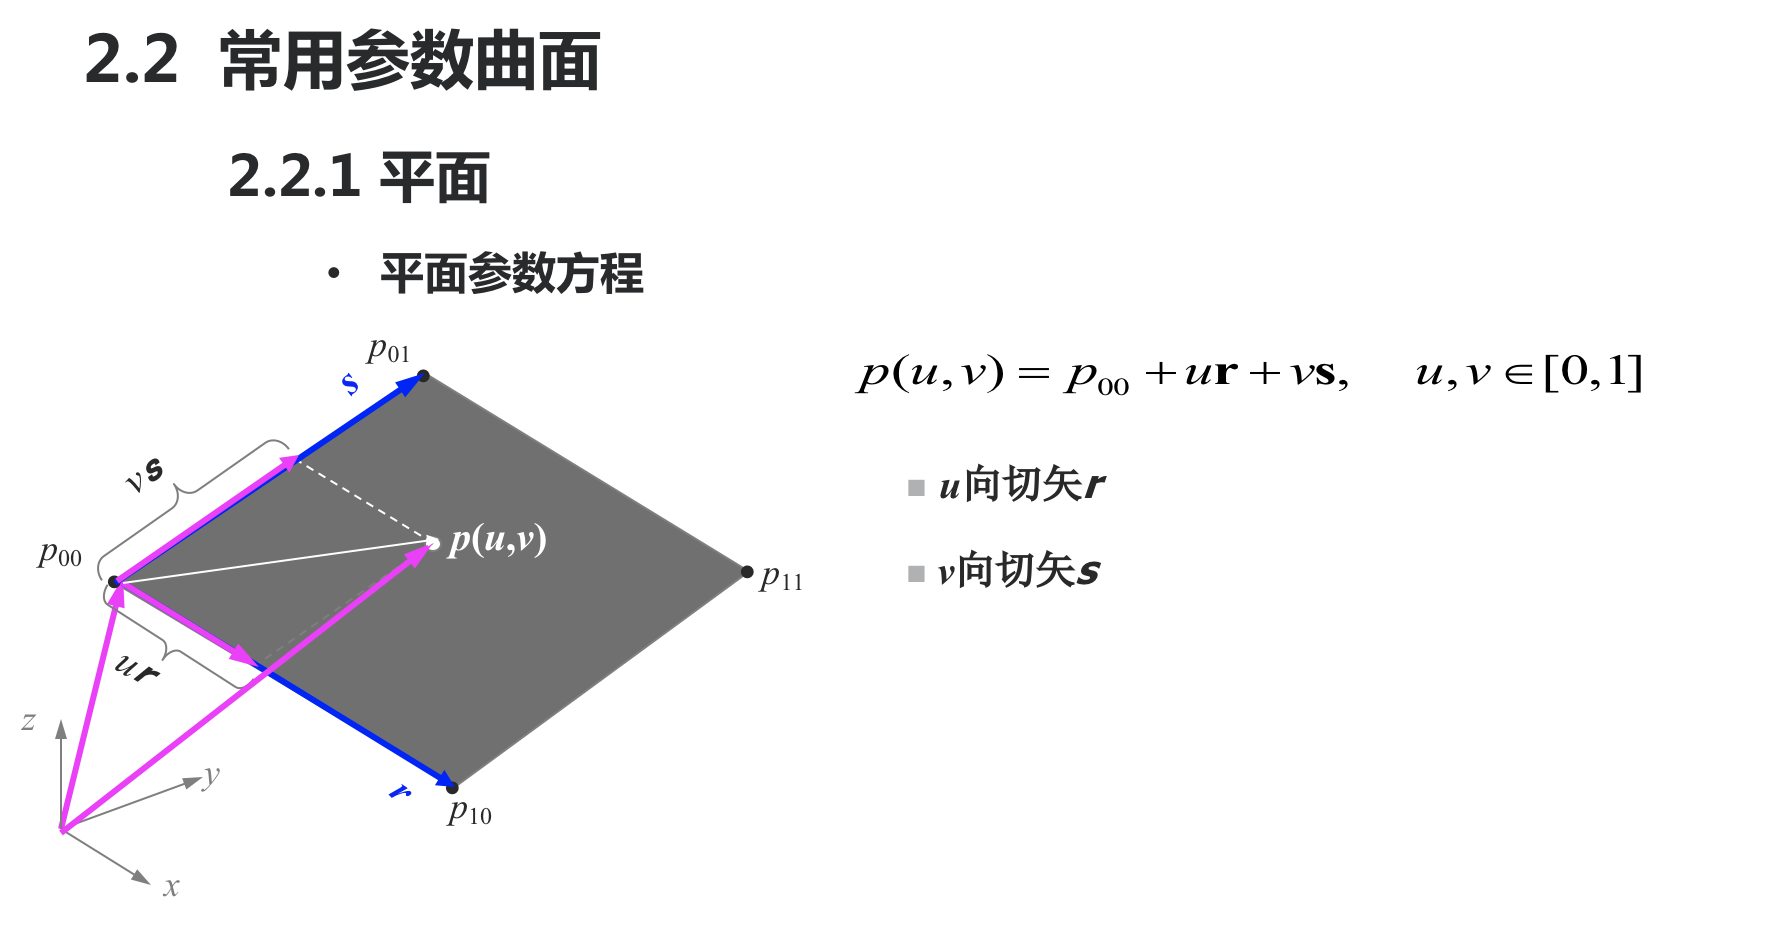
\includegraphics{/Users/yue/Documents/GitHub/2019-2020-autumn-semester/SE-344/submissions/ass4-ng-x/notes/12-05.assets/image-20191229163448367.png}
\caption{}
\end{figure}

平面就是简单的线性比例加和。手指头就能想明白。

\hypertarget{header-n95}{%
\subparagraph{直纹面}\label{header-n95}}

\begin{figure}
\centering

\includegraphics{/Users/yue/Documents/GitHub/2019-2020-autumn-semester/SE-344/submissions/ass4-ng-x/notes/12-05.assets/image-20191229163723607.png}
\caption{}
\end{figure}

\begin{quote}
啥是直纹面啊?
\end{quote}

在\href{https://zh.wikipedia.org/wiki/幾何學}{幾何學}中,如果一個曲面上的任意一點上均有至少一條\href{https://zh.wikipedia.org/wiki/直線}{直線}經過,則稱該曲面為\textbf{直紋曲面}。另一種常見的說法是,如果一個曲面可以由一條直線通過連續運動構成,則可稱其為直紋曲面。

\begin{figure}
\centering
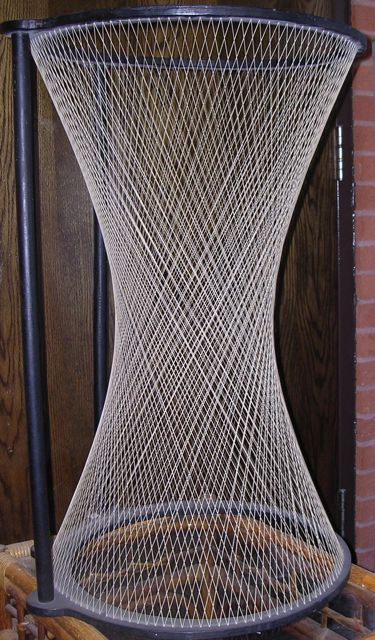
\includegraphics{/Users/yue/Documents/GitHub/2019-2020-autumn-semester/SE-344/submissions/ass4-ng-x/notes/12-05.assets/Ruled_hyperboloid.jpg}
\caption{}
\end{figure}

比如很好看的单叶双曲面就是直纹面。

\hypertarget{header-n102}{%
\subparagraph{双线性曲面}\label{header-n102}}

\begin{figure}
\centering

\includegraphics{/Users/yue/Documents/GitHub/2019-2020-autumn-semester/SE-344/submissions/ass4-ng-x/notes/12-05.assets/image-20191229163957545.png}
\caption{}
\end{figure}

根据这个想象一下,相当于把 \(u\)、\(v\) 的 0 ~ 1 取值范围给 Map
到了四个 P 对应的四边形里了\ldots{}

矩阵表示看起来是真漂亮。

\hypertarget{header-n106}{%
\subparagraph{Linear Coons Curve}\label{header-n106}}

\hypertarget{header-n107}{%
\subparagraph{Type II Coons Curve}\label{header-n107}}

\hypertarget{header-n108}{%
\subparagraph{Bezier 曲面}\label{header-n108}}

\begin{figure}
\centering

\includegraphics{/Users/yue/Documents/GitHub/2019-2020-autumn-semester/SE-344/submissions/ass4-ng-x/notes/12-05.assets/image-20191229164340099.png}
\caption{}
\end{figure}

控件中的一堆点组成点列来决定曲面。

这时候不像二维的控制柄了,这会儿控制柄进化为一个控制网格,每一个点对应网格中的一个小面片。

\hypertarget{header-n112}{%
\subparagraph{B 样条曲面}\label{header-n112}}

\begin{figure}
\centering

\includegraphics{/Users/yue/Documents/GitHub/2019-2020-autumn-semester/SE-344/submissions/ass4-ng-x/notes/12-05.assets/image-20191229164502947.png}
\caption{}
\end{figure}

\hypertarget{header-n114}{%
\subparagraph{NURBS}\label{header-n114}}

\begin{figure}
\centering

\includegraphics{/Users/yue/Documents/GitHub/2019-2020-autumn-semester/SE-344/submissions/ass4-ng-x/notes/12-05.assets/image-20191229164539200.png}
\caption{}
\end{figure}

\hypertarget{header-n116}{%
\subparagraph{扫描面}\label{header-n116}}

Swept Surface...

这个很有意思了。

\begin{figure}
\centering
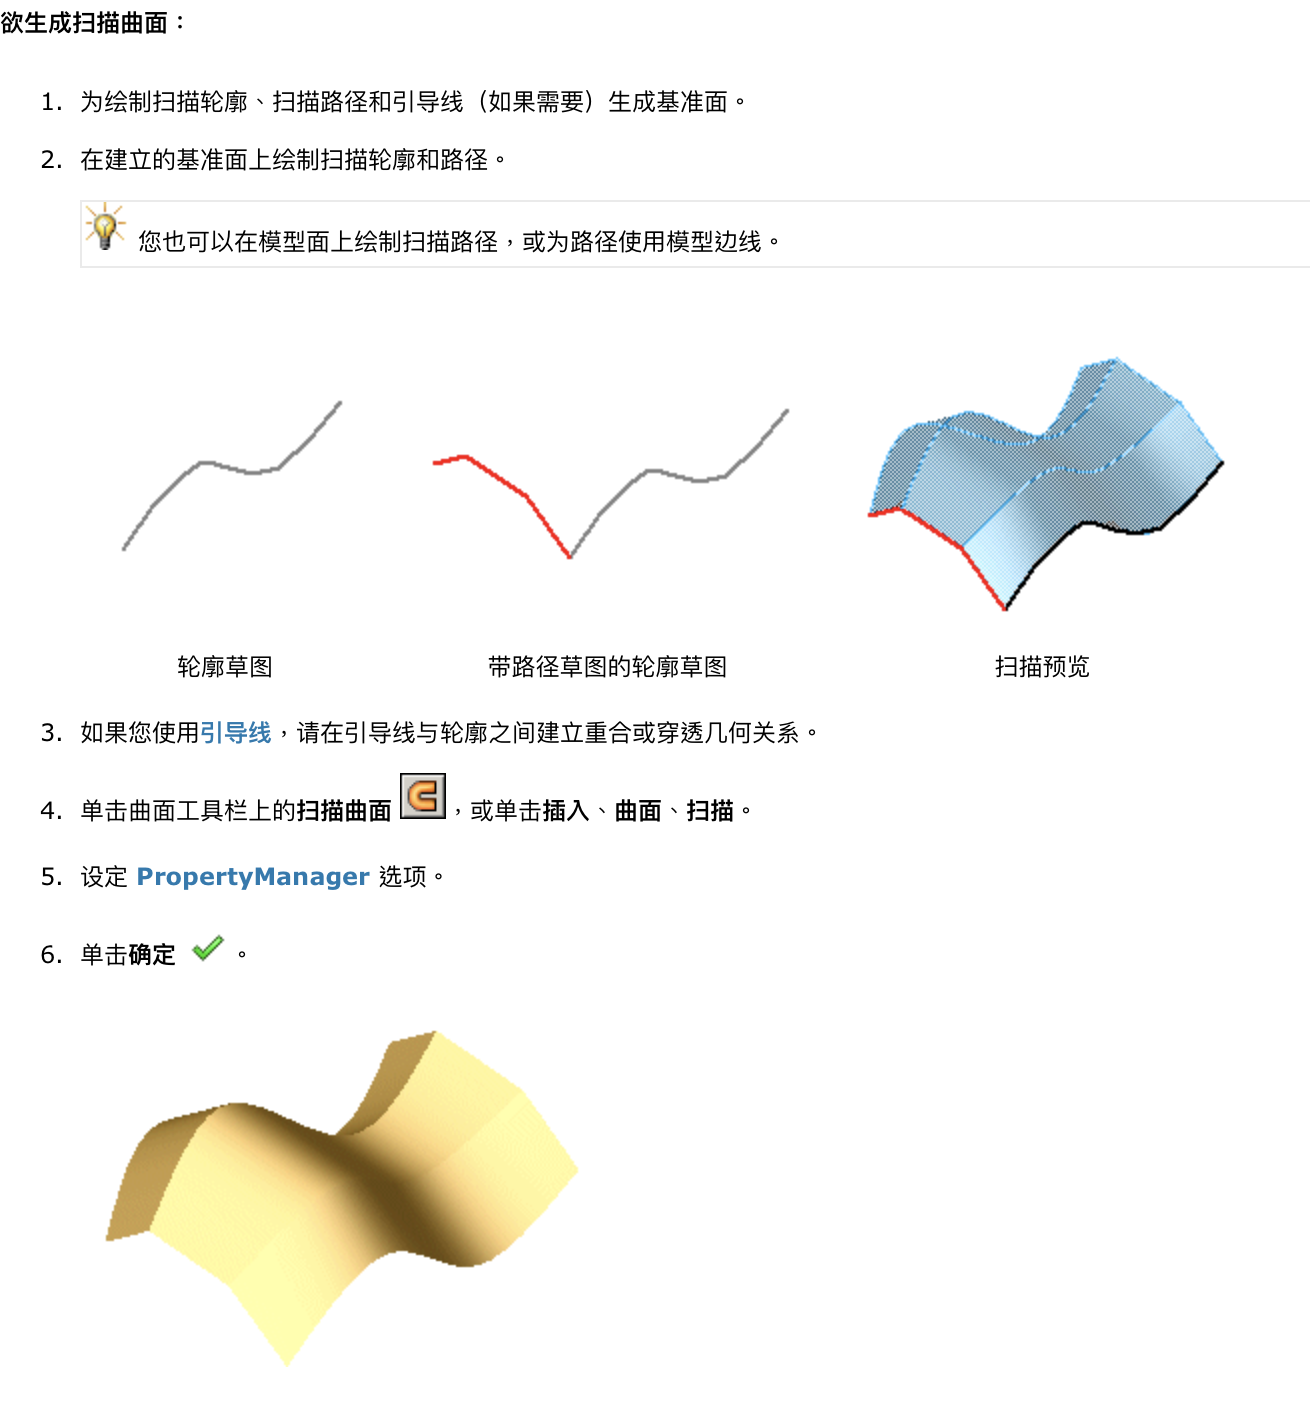
\includegraphics{/Users/yue/Documents/GitHub/2019-2020-autumn-semester/SE-344/submissions/ass4-ng-x/notes/12-05.assets/image-20191229164254491.png}
\caption{}
\end{figure}

用两个正交平面上的曲线来构造出一个曲面,结果灵活而直观。

\hypertarget{header-n121}{%
\subsubsection{OpenGL APIs}\label{header-n121}}

跟二维里一个套路\ldots 用 \texttt{glMap2}
造出一个求值器,然后只要按照一定的密度调用求值函数,它就会帮你用 (u, v)
吐出一堆 (x, y, z)。

可以通过 \texttt{glEvalCoord2} 来计算单个顶点,也可以用
\texttt{glMapGrid2} 和 \texttt{glEvalMesh2} 来计算均匀曲面的坐标。

你拿到顶点之後,再用这个来画图就得了。

\end{document}
